\chapter{Continental}\label{chapConti}
\putminitoc
Mon stage s'est déroulé au sein de l'entreprise Continental. Cette entreprise est, sur les dernières années, entre première et deuxième équipementier automobile mondial par le volume de vente.

Ce chapitre présente rapidement le groupe Continental et plus particulièrement l'équipe \textit{Tests \& Automation Service} qui m'a accueilli pour ce stage.

	\section{Organisation de l'entreprise}
		\subsection{Le groupe Continental}

Continental est une entreprise allemande fondée en 1871 dont le siège se situe à Hanovre. Il s'agit d'une Société Anonyme (SA) dont le président du comité de
direction est le Dr. Elmar \bsc{Degenhart} depuis le 12 août 2009. Le groupe Continental est constitué de cinq divisions intervenant sur le marché des pneus (\textit{Rubben}) et de l'électronique automobile (\textit{Automotive}), ces divisions vous sont détaillés figure \ref{fig:repartitionConti}.
	 
		 \begin{figure}[H]
		 	\centering
		 	\includegraphics[width=17cm]{contents/images/caConti.png}
		 	\caption[Chiffre d'affaire et nombre d'employes (Annee 2014)]{Chiffre d'affaire et nombre d'employes (Annee 2014)\footnotemark{}}
		 	\label{fig:caConti}
		 \end{figure}
	 	\footnotetext{NAFTA : North American Free Trade Agreement}
		 En 2014, l'entreprise comptait plus de $189\;000$ employés dans le monde, comme le montre la figure\ref{fig:caConti} répartis dans 317 sites et 50 pays différents, dont la répartition est détaillée figure \ref{fig:repartitionConti}. Avec un chiffre d'affaire de 34.5 milliards d'euros au total, Continental est le numéro un du marché de production de pneus en Allemagne et est également un important équipementier automobile.

		 \begin{figure}[H]
		 	\centering
		 	\includegraphics[width=18cm]{contents/images/repartitionConti.png}
		 	\caption{Répartition du groupe Continental dans le monde}
		 	\label{fig:repartitionConti}
		 \end{figure}		 

		\subsection{Histoire de l'entreprise}
		Continental est fondée en 1871 comme société anonyme sous le nom de <<\textit{Continental-Caoutchouc-und Gutta-Percha Compagnie}>> par neuf banquiers et industriels de Hanovre (Allemagne).

		Continental dépose l'emblème du cheval représenté sur la figure \ref{fig:logo}, comme marque de fabrique à l'Office impérial des brevets de Hanovre en octobre 1882. Ce logo est aujourd'hui encore protégé en tant que marque distinctive.
		\begin{figure}[H]
			\centering
			\includegraphics[width=3cm]{contents/images/logoConti.png}
			\caption{Logo de Continental}
			\label{fig:logo}
		\end{figure}

		Le fabricant de pneus allemand débute son expansion à l'international en tant que sous-traitant automobile international en 1979, expansion qu'il n'a cessé de poursuivre depuis.
		
Entre 1979 et 1985, Continental procède à plusieurs rachats qui permettent son essor en Europe, celui des activités pneumatiques européennes de l'américain \textit{Uniroyal Inc.} et celui de l'autrichien \textit{Semperit}.

En 1995 est créée la division << \textit{Automotive Systems} >> pour intensifier les activités << systèmes >> de son industrie automobile.

La fin des années 1990 marque l'implantation de Continental en Amérique latine et en Europe de l'Est.

En 2001, pour renforcer sa position sur les marchés américain et asiatique, l'entreprise fait l'acquisition du spécialiste international de l'électronique \textit{Temic}, qui dispose de sites de production en Amérique et en Asie. La même année, la compagnie reprend la majorité des parts de deux entreprises japonaises productrices de composants d'actionnement des freins et de freins à disques. 

En 2004, le plus grand spécialiste mondial de la technologie du caoutchouc et des plastiques naît de la fusion entre \textit{Phoenix AG} et \textit{Conti'Tech}.

Enfin en juillet 2007, Continental réalise sa plus grosse opération en rachetant le fournisseur automobile \textit{Siemens VDO Automotive}. Ce rachat a permis à l'entreprise de multiplier son chiffre d'affaire par deux, passant ainsi de 13 milliards d'euros à plus de 34.5 milliards d'euros (chiffre de 2014).
		
		\subsection{Activités des différentes branches}
		\begin{figure}[H]
			\hspace{-55px}
			\includegraphics[width=21cm]{contents/images/structureConti.jpg}
			\caption{Structure de Continental}
			\label{fig:structConti}
		\end{figure}

		Comme on peut le voir sur la figure \ref{fig:structConti}, Continental est composée de cinq divisions. Ces dernières se chargent de développer et produire des équipements répondant aux besoins des clients. Pour cela elles sont composées de \textit{Business Units} qui ont chacune une activité bien particulière dans leur domaine de compétence. 

Durant mon stage, je travaillais au sein de \textit{P-ES} : 
\begin{description}
	\item[Division \textit{Powertrain}] S'occupe essentiellement du contrôle moteur, au niveau logiciel et matériel avec l'ECU\footnote{Engine Control Unit, Unité de calcul du contrôle moteur}
	\item[Business Unit \textit{Engine Systems}] Chargée de produire les équipements nécessaires au contrôle moteur tels que des calculateurs ou des injecteurs.
\end{description}

	\section{Le contexte de l'équipe TAS}
		J'ai travaillé dans l'équipe en charge des tests au niveau système ou logiciel dirigée par Corinne \bsc{Tarin}. Cette équipe doit aider à la vérification et la validation des programmes de contrôle moteur en fournissant des services de tests. 
		
 		\subsection{Le besoin} \label{besoinTests}
 		Le calculateur du contrôle moteur d'une voiture est un dispositif très important et à haut risque, en effet, une défaillance peut provoquer la mort de plusieurs personnes\footnote{Le programme d'une voiture comporte ainsi des fonctions dites << \textit{safety} >> tel que le régulateur, l'accélération, le freinage, \ldots}. Ainsi, le test est indispensable dans ce domaine, et doit être robuste. 

Le test des logiciel de contrôle moteur se fait aujourd'hui : 
\begin{itemize}
	\item << Soit à la main >> pour les tests d'intégration
	\item Soit à l'aide de scripts de test Python, écrit manuellement
\end{itemize}
Cependant, la taille des logiciels à tester est devenu particulièrement importante(Plusieurs milliers de variables, dans plus de 10 000 pages de spécifications\ldots). Cela appel à une automatisation plus forte des tests afin d'augmenter fortement la vitesse et la quantité de tests afin d'éliminer le maximum de bogue.

C'est dans ce contexte que l'équipe TAS intervient, c'est ainsi que je participe au développement d'un outil permettant d'automatiser des tests d'intégrations pour les équipes projet travaillant pour Ford.
 		\subsection{L'équipe Tests \& Automation Service}

 		% P : Powertrain
 		% ES : Engine System
 		% SE :
 		% CV :
 		% TAS : Test & Automation Service
 		% TODO ajouter schéma de l'équipe dans Powertrain ?
 		
 		Pour ma part, j'opérais dans la partie test automatique. Cette << sous-équipe >> possède deux missions : 
 		\begin{itemize}
 			\item Le développement et l'exécution de scripts de tests de non-régression\footnote{Aussi appelés FaST : \textbf{F}unctions \textbf{a}nd \textbf{S}oftware \textbf{T}esting}. Ces scripts de tests s'exécutent sur bancs HiL\footnote{\textbf{H}ardware \textbf{I}n the \textbf{L}oop. Vous trouverez plus d'explications sur ce dispositif section \ref{wb}} avant la livraison des projets
 			\item Le développement et la maintenance d'outils permettant d'améliorer la couverture et la qualité des tests. Ces outils doivent permettre aux développeurs de vérifier facilement et correctement leur travail, particulièrement pour des tests de non-régression bien que l'outil sur lequel je travail soit à destination de tests d'intégration.
 		\end{itemize}
	\subsection{Les outils de tests}
	Afin d'effectuer son travail, l'équipe TAS possède différents outils de tests. D'une part au niveau matériel avec des bancs de tests, mais aussi logiciel avec une plateforme écrite en Python.
	
		\subsubsection{Les bancs de tests}\label{wb}
		Afin de tester au mieux les programmes du contrôle moteur développés, ceux-ci sont d'abord testé via des simulateurs d'environnement véhicule. Ce simulateur permet de vérifier le programme avant d'effectuer des tests sur véhicule. Ces tests se font sur table dans un premier temps, pour deux raisons principales : 
		\begin{itemize}
			\item D'un part, les tables sont plus facilement accessible qu'un véhicule d'essais pour les équipes logicielles
			\item D'autre part, les tables possèdent plus de moyens afin d'observer finement l'ECU
		\end{itemize}
		
		Comme vous pouvez le voir figure \ref{fig:wb}, un banc de tests est composé d'un ordinateur, du calculateur appelé ECU pour \textit{\textbf{E}lectronic \textbf{C}ontrol \textbf{U}nit} et d'au moins deux équipements aidant aux tests. 
		
		Les deux équipements étant les suivants : 
		\begin{description}
			\item[Le HiL] Le \textit{\textbf{H}ardware \textbf{i}n the \textbf{L}oop} est un simulateur d'environnement véhicule. Ainsi l'ECU est branché sur le HiL et se comporte de la même manière que s'il était embarqué dans une voiture. Le HiL quant à lui est chargé d'envoyer les bons stimulus sur les pins de l'ECU, tel que l'injection, la vitesse de rotation du moteur, le starter \ldots
			\item[Debugger] Cet {appareil} est connecté au microcontrôleur de l'ECU via un port JTag. Il peut communiquer avec celui-ci afin d'effectuer différentes opérations. Tel que flasher le logiciel à tester, mettre des points d'arrêts sur le code, lire des variables, les modifier, changer des calibrations, \ldots
		\end{description}
	
		\begin{figure}[H]
			\centering
			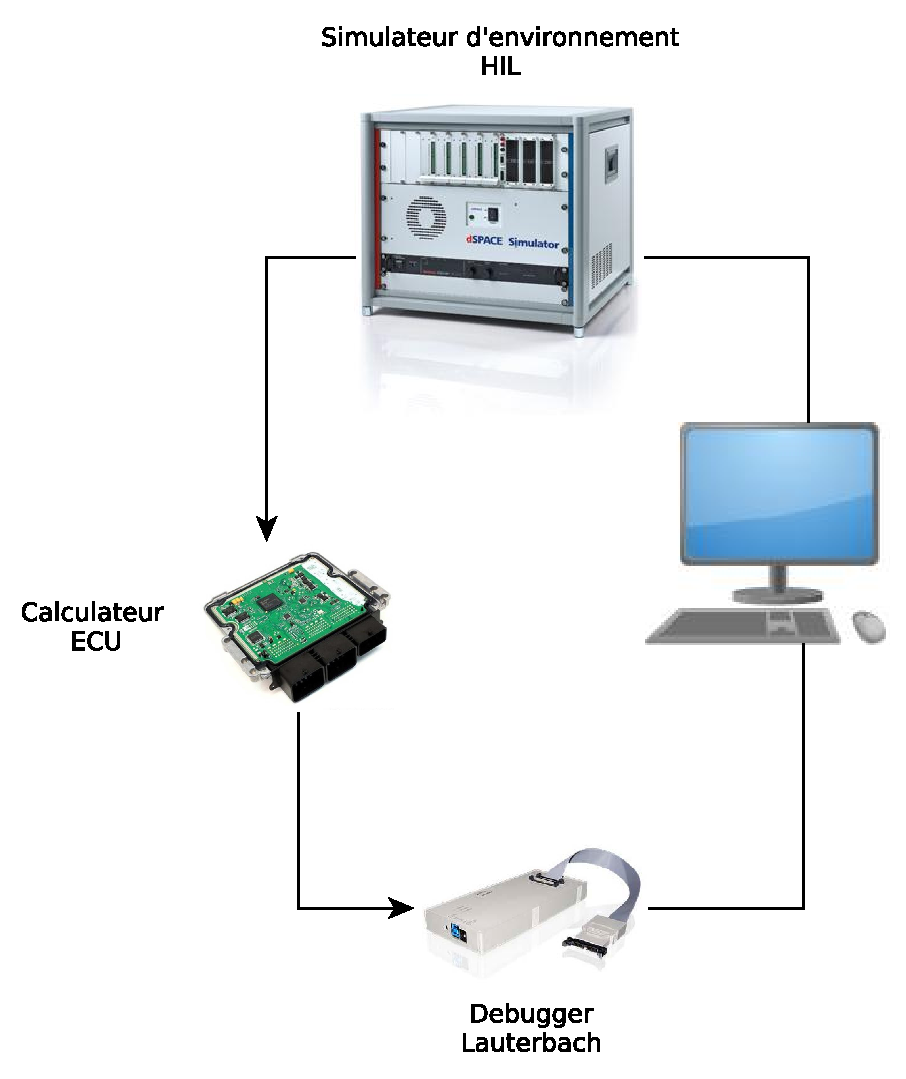
\includegraphics[width=12.1cm]{contents/images/WB.eps}
			\caption{Fonctionnement d'une table de tests : HIL DSpace, Debugger et ECU}
			\label{fig:wb}
		\end{figure}
				\begin{remarque}
					Un certain nombre d'équipes projet chez Continental utilise un troisième équipement qui n'est pas représenté ici, parce que notre plateforme ne s'en sert pas. Cet outil, nommé INCA, va interagir sur l'ECU via un bus CAN\footnote{Controller Area Network}.
				\end{remarque}
		Les différents équipements, ou \textit{device}, que nous pouvons voir sur cette figure sont ceux avec lesquelles notre nouvelle plateforme va communiquer afin d'effectuer des tests automatiques. 
		
			\subsubsection{La plateforme TA3}\label{ta3}
			\begin{wrapfigure}{l}{2.5cm}
				\includegraphics[width=2.5cm]{contents/images/python.png}
			\end{wrapfigure}
			Actuellement, les équipes de tests disposent d'une plateforme appelée TA3. Celle-ci est une bibliothèque de classes écrites en Python. Jusqu'à présent, pour chaque objectif de test, il fallait écrire un script python utilisant la TA3. Ces scripts pilotent le banc HIL et le debugger afin d'envoyer des stimulis à l'unité de contrôle moteur et de vérifier que les réactions de celui-ci sont conforme aux spécifications de test.
			
			Cependant, cette plateforme pose un certain nombre de problèmes qui rend son utilisation difficile. D'une part, elle renvoie un trop grand pourcentage de faux-positifs, faisant perdre du temps au testeur. D'autres part, elle ne prend pas en compte certains besoins apparu récemment comme par exemple un système permettant de flasher automatiquement les ECU\footnote{Cela permettrai de scripter un test qu'on lancerai plus tard et de gagner du temps}, ou la possibilité de vérifier la fréquence de mise-à-jour de la production de variables\footnote{Ceci afin de contrôler le temps réel du calculateur}.
			
			Afin d'améliorer cette situation, l'équipe \textit{Tests \& Automation Service} développe une nouvelle plateforme.
			
%C'est dans ce contexte que l'équipe \textit{Tests \& Automation Service} intervient, elle doit fournir des outils aux développeurs afin de vérifier facilement et correctement leur travail, particulièrement pour des tests de non-régression, bien que l'outil sur lequel je travaille soit à destination de tests d'intégration.
